%%%%%%%%%%%%%%%%%%%%%%%%%%%%%%%%%%%%%%%%%
% baposter Landscape Poster
% LaTeX Template
% Version 1.0 (11/06/13)
%
% baposter Class Created by:
% Brian Amberg (baposter@brian-amberg.de)
%
% This template has been downloaded from:
% http://www.LaTeXTemplates.com
%
% License:
% CC BY-NC-SA 3.0 (http://creativecommons.org/licenses/by-nc-sa/3.0/)
%
%%%%%%%%%%%%%%%%%%%%%%%%%%%%%%%%%%%%%%%%%

%----------------------------------------------------------------------------------------
%	PACKAGES AND OTHER DOCUMENT CONFIGURATIONS
%----------------------------------------------------------------------------------------

\documentclass[landscape,a0paper,fontscale=0.285]{baposter} % Adjust the font scale/size here

\usepackage{graphicx} % Required for including images
\graphicspath{{figures/}} % Directory in which figures are stored

\usepackage{amsmath} % For typesetting math
\usepackage{amssymb} % Adds new symbols to be used in math mode

\usepackage{booktabs} % Top and bottom rules for tables
\usepackage{enumitem} % Used to reduce itemize/enumerate spacing
\usepackage{palatino} % Use the Palatino font
\usepackage[font=small,labelfont=bf]{caption} % Required for specifying captions to tables and figures

\usepackage{hyperref}

\usepackage{multicol} % Required for multiple columns
\setlength{\columnsep}{1.5em} % Slightly increase the space between columns
\setlength{\columnseprule}{0mm} % No horizontal rule between columns

\usepackage{tikz} % Required for flow chart
\usetikzlibrary{shapes,arrows} % Tikz libraries required for the flow chart in the template

\newcommand{\compresslist}{ % Define a command to reduce spacing within itemize/enumerate environments, this is used right after \begin{itemize} or \begin{enumerate}
\setlength{\itemsep}{1pt}
\setlength{\parskip}{0pt}
\setlength{\parsep}{0pt}

}

\definecolor{lightblue}{rgb}{0.145,0.6666,1} % Defines the color used for content box headers

\begin{document}

\begin{poster}
{
headerborder=closed, % Adds a border around the header of content boxes
colspacing=1em, % Column spacing
bgColorOne=white, % Background color for the gradient on the left side of the poster
bgColorTwo=white, % Background color for the gradient on the right side of the poster
borderColor=lightblue, % Border color
headerColorOne=black, % Background color for the header in the content boxes (left side)
headerColorTwo=lightblue, % Background color for the header in the content boxes (right side)
headerFontColor=white, % Text color for the header text in the content boxes
boxColorOne=white, % Background color of the content boxes
textborder=roundedleft, % Format of the border around content boxes, can be: none, bars, coils, triangles, rectangle, rounded, roundedsmall, roundedright or faded
eyecatcher=true, % Set to false for ignoring the left logo in the title and move the title left
headerheight=0.1\textheight, % Height of the header
headershape=roundedright, % Specify the rounded corner in the content box headers, can be: rectangle, small-rounded, roundedright, roundedleft or rounded
headerfont=\Large\bf\textsc, % Large, bold and sans serif font in the headers of content boxes
%textfont={\setlength{\parindent}{1.5em}}, % Uncomment for paragraph indentation
linewidth=2pt % Width of the border lines around content boxes
}
%----------------------------------------------------------------------------------------
%	TITLE SECTION 
%----------------------------------------------------------------------------------------
%
{
\includegraphics[height=4em]{drexel.png}} % First university/lab logo on the left
{\bf\textsc{House in Your Head}\vspace{0.5em}} % Poster title
{\textsc{\{ Sam Bever, Mike Conway, Joe Muoio, Kyle Patron, Kevin Zakszewski\} \hspace{12pt} Drexel University: CCI}} % Author names and institution
{
\includegraphics[height=4em]{drexel.png}} % Second university/lab logo on the right

%----------------------------------------------------------------------------------------
%	OBJECTIVES
%----------------------------------------------------------------------------------------

\headerbox{Objectives}{name=objectives,column=0,row=0}{

The goal of this project is to cater to ALS patients, giving them the ability to be more autonomous. The key features are:

\begin{itemize}
\item Calibration for individual users
\item Intuitive interface with simple selections
\item Allow users with ALS to perform basic household tasks, such as
    \begin{itemize}
        \item Turning lights on and off
        \item Adjusting the thermostat
        \item Controlling the television
    \end{itemize}
\end{itemize}

\vspace{0.3em} % When there are two boxes, some whitespace may need to be added if the one on the right has more content
}

%----------------------------------------------------------------------------------------
%	INTRODUCTION
%----------------------------------------------------------------------------------------

\headerbox{Introduction}{name=introduction,column=1,row=0, aligned=objectives}{

Amyotrophic lateral sclerosis (ALS) (also called ``Lou Gehrig's Disease'') is
a neurodegenerative disease affecting the brain and spinal cord. The motor
neurons progressively degenerate and die off, leading to the loss of muscle
control and death. Affected indivuals suffer a spectrum of symptoms
culminating in total lock-in. In this state, the patient is aware but cannot
move their body in any way. They cannot breathe on their own or even blink
their eyes. Because of this, late-stage ALS patients are unable to interface
with conventional assistive technologies. \cite{ALSsource}
\break
\break
The goal of the project is to build a system which people afflicted with ALS
can use to interact with their houses through the Insteon Home Automation Systems (HAS).
This includes controlling the thermostat, lights, stereo, and television as
well as interfacing with social media. By having a Brain Computer Interface
(BCI) to their automated house, individuals with ALS can still interact with
their environment despite full paralysis.
}

%----------------------------------------------------------------------------------------
%	Architecture
%----------------------------------------------------------------------------------------

\headerbox{System Overview}{name=architecture,column=2,span=2,row=0}{

\begin{multicols}{2}
\vspace{1em}
\begin{center}
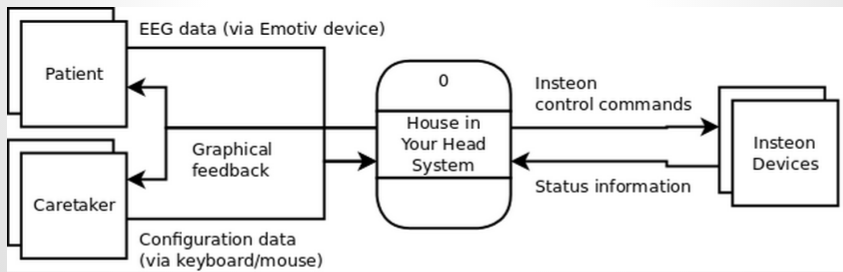
\includegraphics[width=0.8\linewidth]{contextDiagram}
\captionof{figure}{Context Diagram of the system}
\end{center}

The system is broken down into 3 main components. The Graphical User Interface (GUI) component, the electroencephalogram (EEG) processing component, and the Home Automation System (HAS) component. The GUI can be shown on any standard computer display. The GUI scrolls through options one by one until the user makes a selection. This selection is performed by their accept thought. The accept thought is translated to a usable form in the EEG Processing component and can take the form of one of the following: adding numbers, counting, or mentally composing a letter to a friend.
\end{multicols}

%------------------------------------------------

\begin{multicols}{2}
\vspace{1em}
Depending on what is displayed on the GUI at the time of the accept thought, the option is selected and the appropriate call to the HAS component is made. For instance, if the option to turn on a light was shown in the GUI while the user thought their accept thought, the HAS component will receive the instruction to turn on the light which it will then forward the appropriate commands to the Insteon system. This will in turn, turn the light on. 

\begin{center}
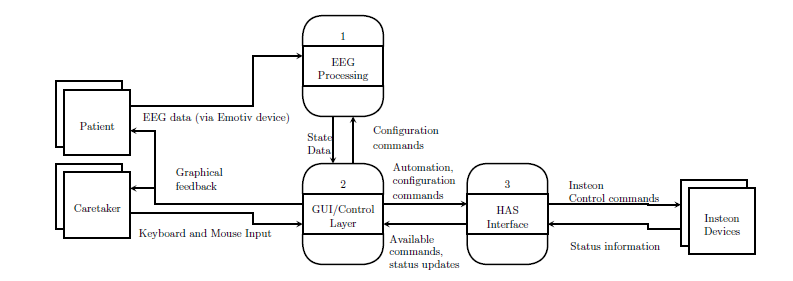
\includegraphics[width=0.8\linewidth]{level0DFD}
\captionof{figure}{Level 0 DFD of the main system components}
\end{center}

\end{multicols}
}

%----------------------------------------------------------------
% PROGRAM FLOW
%-----------------------------------------------------------------
\headerbox{Program Flow}{name=flow,column=0,row=1,below=objectives}{

At the application selection screen  (\autoref{fig:ui}), the user will cycle through the options of the objects that they can interact with in the home automation system. This is also the screen where the user decides which object they want to interact with. When an object is chosen, the user will be directed to the interactive state screen for the selected object. This screen handles the changing of the state of the object the user selects. This could be some as simple as a state change from "on" to "off" or input that requires integer input (\autoref{fig:integerInput}) From this screen the user can either change the state or return to the previous screen (the first type where the users cycle through the options). These three types of UI screens will make up the majority of the user interaction in the system. These designs will be modified or extra user interface designs will be implemented as necessary. 
}


\headerbox{Program Flow Image}{name=flowimage,column = 1, below=introduction}{

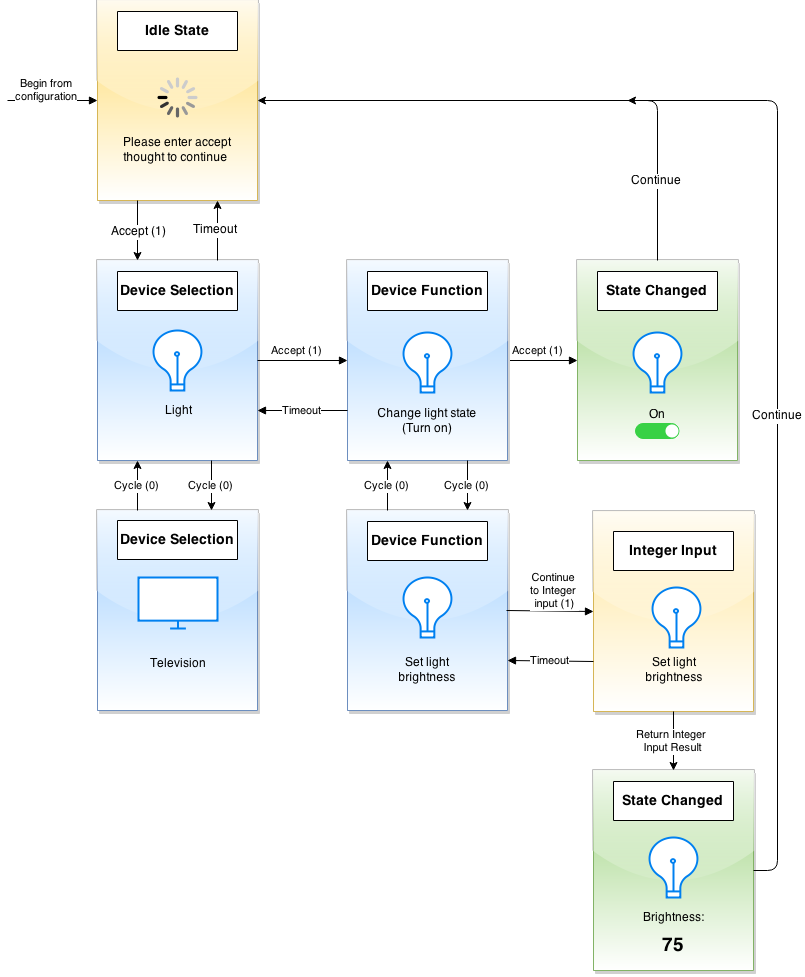
\includegraphics[width=0.8\linewidth]{ApplicationUI}
\captionof{figure}{General flow of the program}

}

%----------------------------------------------------------------------------------------
%	REFERENCES
%----------------------------------------------------------------------------------------

\headerbox{References}{name=references,column=2,row=2,above=bottom}{
\begin{thebibliography}{1}
    \bibitem{ALSsource} The ALS Association. (2014, October, 5). \textit{What
        is ALS?} [Online]. Available:
        \url{http://www.alsa.org/about-als/what-is-als.html}
 
    \bibitem{Emotiv} Emotiv, Inc. (2015, May, 5). \textit{Emotiv|EEG
        System} [Online]. Available: \url{http://emotiv.com/}
        
    \bibitem{Insteon} Insteon \textregistered. (2015, May, 5). \textit{Insteon} [Online]. Available: \url{http://www.insteon.com/}
\end{thebibliography}
}

%----------------------------------------------------------------------------------------
%	FUTURE RESEARCH
%----------------------------------------------------------------------------------------

\headerbox{Future Work}{name=futureresearch,column=0,span=1,above=bottom}{ % This block is as tall as the references block

\begin{itemize}\compresslist
\item More devices can be tested with the HAS. (ie: anything using an IR sensor)
\item The UI can be expanded to work with multiple inputs instead of just a singular brain input
\item Better methods of machine learning can be tried
\end{itemize}
}

%----------------------------------------------------------------------------------------
%	CONTACT INFORMATION
%----------------------------------------------------------------------------------------

\headerbox{Contact Information}{name=contact,column=3,aligned=futureresearch,above=bottom}{ % This block is as tall as the references block

\begin{description}\compresslist
\item[Email] jgm55@drexel.edu
\item[url] http://drexel.edu/cci/resources/current-students/undergraduate/senior-design-challenge/
\item
\end{description}
}

%----------------------------------------------------------------------------------------
%	CONCLUSION
%----------------------------------------------------------------------------------------

\headerbox{Conclusion}{name=conclusion,column=2,span=2,row=0,below=architecture,above=references}{

%------------------------------------------------

\begin{itemize}\compresslist
\item Patients with ALS can achieve a huge quality of life improvement with a BCI by automating their house
\item The UI supports house automation through the input of the Emotiv Headset
\item We showed that the Insteon home automation system can be used without movement from the user.
\end{itemize}
}

%----------------------------------------------------------------------------------------

\end{poster}

\end{document}